\documentclass[11pt,a4paper]{article}
\usepackage[utf8]{inputenc}
\usepackage[T1]{fontenc}
\usepackage[brazil]{babel}
\usepackage{lmodern}
\usepackage[margin=2cm]{geometry}
\usepackage{amsmath,amssymb}
\usepackage{booktabs}
\usepackage{graphicx}
\usepackage{hyperref}
\usepackage{xcolor}
\usepackage{titlesec}
\usepackage{tabularx}
\usepackage{enumitem}
\usepackage{float}

\hypersetup{
    colorlinks=true,
    linkcolor=blue!70!black,
    citecolor=blue!70!black,
    urlcolor=blue!70!black
}

\titleformat{\section}{\large\bfseries}{\thesection.}{0.5em}{}
\titleformat{\subsection}{\normalsize\bfseries}{\thesubsection.}{0.5em}{}
\titlespacing*{\section}{0pt}{1.2ex plus 0.5ex minus .2ex}{0.6ex}
\titlespacing*{\subsection}{0pt}{1.0ex plus 0.4ex minus .2ex}{0.4ex}

\setlength{\parskip}{0.45em}
\setlength{\parindent}{0pt}
\setlist{itemsep=0.15em,topsep=0.3em}

\begin{document}

\begin{center}
    {\LARGE \textbf{Relatório de Status do TCC}} \\[0.35em]
    {\large Avaliação das Explicações SHAP em Redes Neurais Profundas para Classificação de Arritmias Cardíacas em ECG} \\[0.3em]
    \textbf{Aluno:} Arthur Santos de Oliveira (RA: 156297) \\[0.2em]
    \textbf{Orientador:} Prof.\ Dr.\ Luis Augusto Martins Pereira \\[0.2em]
    \textbf{Período:} 30/09/2026 a 09/10/2026 \\[0.2em]
    \textbf{Repositório:} \url{https://github.com/Arthur-so/shap-ecg-arrhythmia}
\end{center}
\vspace{-0.5em}
\hrule
\vspace{0.8em}

\section{Resumo do período}

\begin{itemize}
    \item Leitura do artigo que define as métricas \textit{Consistency} e \textit{Sufficiency} (Dasgupta, Frost e Moshkovitz, 2022) e análise do que se aplica a explicações SHAP de ECG.
    \item \textit{Sufficiency} retirada da análise, por não ter definição no artigo para métodos de importância de atributos.
    \item Identificação de um defeito na \textit{Consistency} do Quantus e implementação própria da métrica, fiel ao artigo e adaptada ao ECG.
    \item Correção de uma falha de rotulagem que deixava a classe CVP sem nenhuma amostra.
    \item Alinhamento do treino ao protocolo do artigo base (Zhang et al., 2021): F1-macro no teste passou de 0,641 para \textbf{0,819} (artigo: 0,813).
    \item Geração das explicações SHAP do novo modelo, cálculo da \textit{Consistency} e primeiras conclusões.
\end{itemize}

\section{Leitura de Dasgupta et al. (2022): o que se aplica ao trabalho}

O artigo define a fidelidade de uma explicação ao modelo por meio de duas propriedades complementares:
\begin{itemize}
    \item \textbf{Consistency:} instâncias que recebem a \emph{mesma explicação} devem receber a mesma predição.
    \item \textbf{Sufficiency:} se a propriedade apontada pela explicação de $x$ também está presente em outra instância $x'$, então $x'$ deve receber a mesma predição, mesmo que a explicação de $x'$ seja outra.
\end{itemize}

\textbf{O que se aplica.} A \textit{Consistency} se aplica a mapas SHAP desde que eles sejam \emph{discretizados}: mapas contínuos de $12 \times 15000$ valores nunca se repetem, e o artigo propõe reduzi-los a uma representação simplificada (por exemplo, o sinal dos atributos de maior importância) antes de comparar (p.~11 e Apêndice D.5).

\textbf{Por que a \textit{Sufficiency} foi retirada.} Os próprios autores afirmam que, para métodos de importância de atributos (SHAP, LIME, gradiente), não está claro quando uma explicação ``se aplica'' a outra instância, e por isso analisam apenas a \textit{Consistency} nesses métodos (p.~8). A versão do Quantus contorna isso comparando mapa com mapa por distância, o que na prática é uma \textit{Consistency} relaxada, e não a \textit{Sufficiency} do artigo. Por não ter base na definição original, a métrica foi deixada de fora.

\section{Consistency: defeito no Quantus e implementação própria}

\textbf{Defeito encontrado.} A discretização padrão da \texttt{quantus.Consistency} (v0.6.0) toma o sinal dos 5 \emph{primeiros} valores do mapa, e não dos 5 mais importantes, depois de aplicar valor absoluto. Nos mapas do projeto, isso produziu \textbf{a mesma explicação para todos os ECGs}, em todas as classes (verificado nos mapas). A métrica passava a medir só a homogeneidade das predições dentro de cada classe, e por isso acompanhava o F1 de forma mecânica.

\textbf{Implementação própria} (\texttt{src/consistency.py}), seguindo a definição e o estimador do artigo:
\begin{enumerate}
    \item \textbf{Regiões do batimento:} o ECG tem 12 derivações, registradas ao mesmo tempo, e o mapa SHAP tem um valor para cada derivação e cada instante. Os picos R (o pico do complexo QRS de cada batimento) são localizados em uma das derivações, a derivação II, com a biblioteca NeuroKit2. Como as 12 derivações são simultâneas, os mesmos instantes valem para todas elas. Cada batimento (o trecho entre dois picos R consecutivos) é então dividido em três regiões (Figura~\ref{fig:regioes}): \textbf{QRS} (de 80~ms antes a 100~ms depois do R), \textbf{ST-T} (do fim do QRS até 45\% do intervalo RR) e \textbf{pré-QRS} (o restante, que contém a onda P e o intervalo PR). O trecho de preenchimento (\textit{padding}) é excluído. A localização exata de P, QRS e T foi testada e descartada, porque falhou justamente nas classes de interesse (``onda P'' detectada na fibrilação atrial e QRS largo não detectado nos bloqueios de ramo).
    \item \textbf{Resumo do mapa:} a atribuição SHAP é somada por derivação $\times$ região, o que dá 36 valores por mapa.
    \item \textbf{Discretização:} dos 36 valores, mantêm-se apenas as $k$ regiões de maior importância em valor absoluto, junto com o sinal de cada uma (+ quando a região contribui a favor da classe explicada, $-$ quando contribui contra). O parâmetro $k$ é, portanto, \textbf{quantas regiões compõem a explicação}. Com $k = 2$, a explicação de um ECG é o par das duas regiões mais importantes, por exemplo ``V1·QRS (+) e V2·QRS (+)''; dois ECGs têm a mesma explicação quando coincidem essas duas regiões e seus sinais. É o análogo ao \textit{Sign-of-top-5} do artigo, que usa os 5 atributos mais importantes. A escolha de $k$ é um compromisso: $k$ pequeno gera explicações pobres, que se repetem entre classes diferentes; $k$ grande gera explicações tão específicas que muitos mapas ficam sem nenhum outro igual e não podem ser avaliados (o estimador do artigo lhes atribui 0). Foi usado $k = 2$ e, para comparação, $k = 1$ e $k = 3$ (seção~\ref{sec:resultados}).
    \item \textbf{Estimador:} todos os mapas, de todas as classes, são agrupados pela explicação discretizada. Para cada mapa, calcula-se a fração dos \emph{outros} mapas do seu grupo que explicam a mesma classe que ele. Por exemplo, se um mapa de BRD tem a explicação ``V1·QRS (+) e V2·QRS (+)'' e outros 10 mapas têm essa mesma explicação, dos quais 8 são de BRD, o valor desse mapa é 8/10 = 0,8. Um mapa é \textbf{sem par} quando nenhum outro mapa tem a mesma explicação que ele, ou seja, quando está sozinho no seu grupo. Nesse caso não há com o que comparar, e o estimador do artigo lhe atribui 0 (a fidelidade não pode ser verificada). A \textit{Consistency} de uma classe é a média dos valores dos seus mapas.
\end{enumerate}

\begin{figure}[H]
\centering
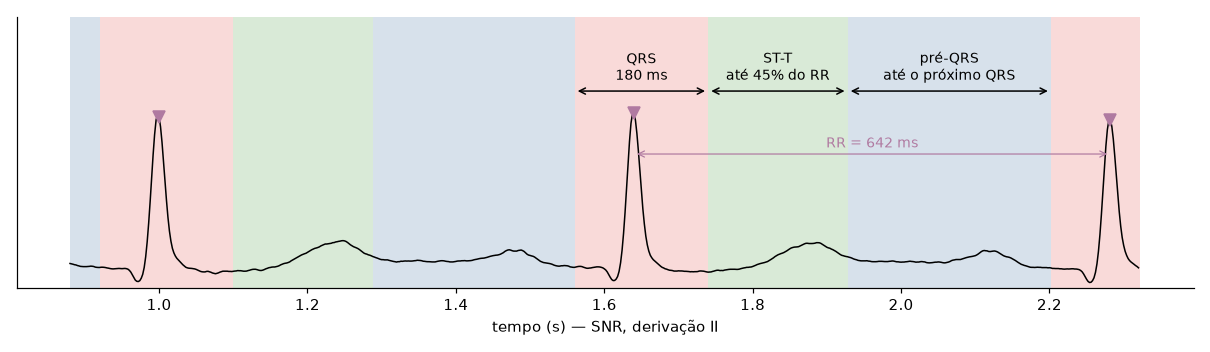
\includegraphics[width=0.92\textwidth]{figs/batimento.png}
\caption{Trecho de cerca de 1,5~s da derivação II de um ECG normal (SNR), com três picos R marcados (triângulos) e as regiões de cada batimento: QRS (vermelho), ST-T (verde) e pré-QRS (azul). A derivação II é usada apenas para localizar os picos R; as mesmas regiões são aplicadas às 12 derivações.}
\label{fig:regioes}
\end{figure}

\textbf{Conferência do código.} Para garantir que a implementação calcula o que deveria, foram feitas duas checagens: (i) antes de escrever o módulo definitivo, a métrica foi calculada com um script provisório; os dois, rodados sobre os mesmos mapas, deram resultados idênticos; (ii) o valor esperado ao acaso, apresentado na seção~\ref{sec:resultados}, é obtido por uma fórmula; para conferi-la, as classes foram embaralhadas entre os mapas 3000 vezes, a \textit{Consistency} foi recalculada em cada embaralhamento, e a média coincidiu com a fórmula.





\section{Correções e melhoria do classificador}

\textbf{Classe CVP sem amostras.} Os registros de extrassístole ventricular usam o código SNOMED \texttt{164884008}, que não estava no mapeamento de rótulos. Com isso, 607 registros ficavam sem rótulo e entravam no treino como ``nenhuma classe''. O código foi adicionado, e todos os 6877 registros passaram a ter rótulo.

\textbf{F1 abaixo do artigo base.} O código foi comparado com o artigo e com a implementação pública dos autores, e foram corrigidos: taxa de aprendizado (1e-3 $\rightarrow$ 1e-4), kernel dos blocos residuais (3 $\rightarrow$ 7), \textit{pooling} final (média $\rightarrow$ média + máximo), aumento de dados (escala e deslocamento de linha de base) e \textbf{limiar de decisão por classe} otimizado no F1 da validação.

\textbf{Ablação da função de perda.} A BCE ponderada por classe (prevista na proposta) foi comparada com a BCE simples (usada pelos autores), em 60 épocas. Os resultados foram equivalentes (Tabela~\ref{tab:f1}), e adotou-se a \textbf{BCE simples}, por ser mais fiel à referência, gerar probabilidades mais bem calibradas e convergir mais rápido. \textit{Esta é uma mudança em relação à seção 4.2 da proposta.}

\begin{table}[h]
\centering
\small
\caption{Evolução do F1-macro no conjunto de teste.}
\label{tab:f1}
\begin{tabularx}{\textwidth}{lXc}
\toprule
\textbf{Versão} & \textbf{O que mudou} & \textbf{F1 teste} \\
\midrule
Run 1 & Classe CVP sem rótulo; lr 1e-3, kernel 3, limiar 0,5 & 0,590 \\
Run 2 & CVP corrigida & 0,641 \\
Run 3 & Treino alinhado ao artigo, BCE ponderada, 40 épocas & 0,803 \\
A & Run 3 com 60 épocas, BCE ponderada & 0,816 \\
\textbf{B (escolhido)} & \textbf{Run 3 com 60 épocas, BCE simples} & \textbf{0,819} \\
\midrule
Zhang et al. (2021) & Média de 10 \textit{folds} & 0,813 \\
\bottomrule
\end{tabularx}
\end{table}

\section{Resultados da Consistency (modelo B)}
\label{sec:resultados}

Foram geradas explicações GradientSHAP para as 622 predições corretas do teste. A \textit{Consistency} global foi \textbf{0,42}, contra 0,13 esperado ao acaso. A Tabela~\ref{tab:cons} mostra os valores por classe, e a Figura~\ref{fig:disp}, a comparação com o F1.

\textbf{Valor esperado ao acaso.} É a \textit{Consistency} que se obteria se as explicações não tivessem nenhuma relação com a classe, como se as classes fossem sorteadas entre os mapas. Ele serve só como referência para saber se um valor é alto ou baixo; nada é descontado. Não é zero porque, mesmo com explicações sorteadas, dois mapas com a mesma explicação às vezes seriam da mesma classe por coincidência, e isso acontece mais nas classes grandes. Por exemplo, 172 dos 622 mapas (28\%) são de BRD, e o acaso dessa classe é 0,23; já o STE tem 14 mapas, e o acaso dele é 0,02. Assim, o BRD, com 0,64, está bem acima do acaso, enquanto o STE, com 0,03, está praticamente nele.

\begin{table}[h]
\centering
\small
\caption{F1 e \textit{Consistency} ($k = 2$) por classe, modelo B, ordenados pela \textit{Consistency}.}
\label{tab:cons}
\begin{tabular}{lrrrrl}
\toprule
\textbf{Classe} & \textbf{Mapas} & \textbf{F1} & \textbf{Consistency} & \textbf{Acaso} & \textbf{Explicação mais comum} \\
\midrule
BRD  & 172 & 0,927 & 0,64 & 0,23 & V1·QRS + V2·QRS \\
STD  &  65 & 0,778 & 0,51 & 0,09 & II·ST-T + aVR·ST-T \\
IAVB &  61 & 0,884 & 0,45 & 0,08 & II·pré-QRS + aVR·pré-QRS \\
AF   & 108 & 0,931 & 0,42 & 0,14 & V4·QRS + V5·QRS \\
CVP  &  59 & 0,837 & 0,26 & 0,08 & aVR·QRS + V5/aVF·QRS \\
BRE  &  20 & 0,870 & 0,25 & 0,03 & V1·QRS + V2·QRS \\
SNR  &  78 & 0,796 & 0,21 & 0,10 & aVR·pré-QRS + V1·QRS \\
CAP  &  45 & 0,750 & 0,14 & 0,06 & dispersa \\
STE  &  14 & 0,596 & 0,03 & 0,02 & pré-QRS (esperado: ST-T) \\
\bottomrule
\end{tabular}
\end{table}

\begin{figure}[H]
\centering
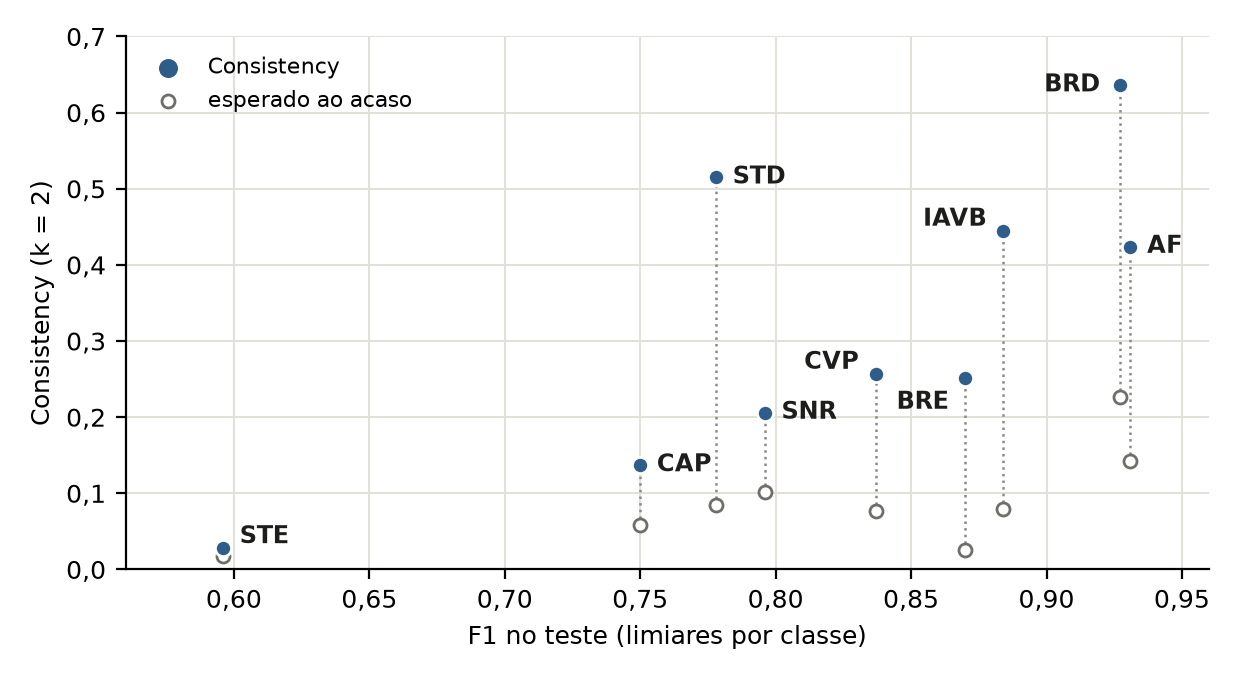
\includegraphics[width=0.68\textwidth]{figs/f1_vs_consistency.png}
\caption{F1 $\times$ \textit{Consistency} por classe (modelo B). Os círculos vazios indicam o valor esperado ao acaso, e a haste, o quanto cada classe fica acima dele.}
\label{fig:disp}
\end{figure}

\textbf{Sensibilidade.} O método foi recalculado com 9 combinações de regiões (janela do QRS de 140, 180 ou 220~ms e fim do ST-T em 40, 45 ou 50\% do RR) e com $k \in \{1, 2, 3\}$. Com $k = 2$, o BRD fica em 1º e CAP e STE nas duas últimas posições em todas as combinações. Com $k = 3$, cerca de 47\% dos mapas ficam sem par (explicação não verificável), e por isso essa opção foi descartada.

\section{Conclusões parciais (apenas F1 e Consistency)}

A comparação com o F1 foi feita de forma \textbf{descritiva} (ordenação e comparação por classe, conforme a seção 4.5 da proposta), sem coeficientes de correlação: as nove classes não são observações independentes (registros multirrótulo, mesmo modelo e mesmo conjunto de teste) nem uma amostra de uma população maior de classes.

\begin{enumerate}
    \item O classificador reproduz o desempenho do artigo base (0,819 contra 0,813). As classes mais difíceis são as mesmas: STE e CAP.
    \item As explicações carregam informação sobre a classe de forma moderada: \textit{Consistency} global de 0,42, cerca de 3 vezes o esperado ao acaso.
    \item A \textit{Consistency} é alta onde o diagnóstico depende de um marcador morfológico localizado (BRD, STD, IAVB), e as regiões destacadas coincidem com os critérios clínicos (QRS em V1 no BRD, ST-T no STD, intervalo PR no IAVB). Isso indica plausibilidade, ainda sem validação por especialista.
    \item Desempenho e consistência coincidem nas pontas: as classes de melhor F1 (BRD, IAVB, AF) estão entre as mais consistentes, e as de pior F1 (CAP, STE) são as menos consistentes. Há exceções no meio (STD com explicações consistentes e F1 intermediário; BRE com bom F1 e explicações pouco consistentes), o que mostra que as duas dimensões não se confundem.
    \item A discretização determina o resultado da métrica: a versão padrão do Quantus gerava uma coincidência artificial com o F1.
\end{enumerate}

\textbf{Limitações:} um único modelo e uma única divisão dos dados; apenas as predições corretas foram explicadas; classes pequenas têm valores pouco estáveis (STE tem 14 mapas); e a \textit{Consistency} mede coerência interna das explicações, e não a sua correção clínica.

\section{Próximos passos}

\begin{itemize}
    \item Ler os artigos das próximas métricas do Quantus, de fidelidade (\textit{Faithfulness Correlation}, \textit{Faithfulness Estimate}, \textit{Sensitivity-N}, \textit{Selectivity}, \textit{Infidelity}) e de robustez (\textit{Local Lipschitz Estimate}, \textit{Max/Avg-Sensitivity}, \textit{Continuity}, RIS e ROS).
    \item Para cada uma, verificar se a implementação do Quantus é aderente à definição original e ao caso de ECG (formato 12 derivações $\times$ 15000 amostras, preenchimento e multirrótulo), como foi feito para a \textit{Consistency}.
    \item Rodar as métricas aderentes sobre o modelo B, resolvendo as pendências de memória já conhecidas (GPU nas métricas de robustez e RAM na \textit{Selectivity}).
\end{itemize}

\textbf{Pontos para discutir com o orientador:} (i) a troca para BCE simples, que difere da proposta; (ii) a análise descritiva sem coeficientes de correlação, que difere do ``calculando a correlação'' da proposta; (iii) a escolha de $k$ ($k = 1$ é mais verificável, com cerca de 2\% dos mapas sem par; $k = 2$ é mais informativo, com cerca de 18\%).

\end{document}
